\chapter{Introduction}
\begin{quote} 
\it This chapter gives a basic introduction to  \ac{DSCs} and \ac{MPPT}.It also defines the scope, Goals, Objective and the Research Methodology for the thesis.
\end{quote}

\section{Background}

Our ever increasing reliance on electrical and electronic equipment intensified our search for new sources of energy. Dwindling fossil-fuel reserves are not something we can rely on in the long-term.Alternate energy sources must be efficient,cost-effective and ecologically friendly.The Harnessing of solar energy becomes a very attractive proposition.A moderately efficient solar cell array (8\%-10\% efficiency) Covering a small portion of the earth's surface would be able to provide an enormous amount of electric power and thus reduce greenhouse-gas emissions \cite{kalyanasundaram2010dye}. However, the current high cost of solar panels made from traditional inorganic semiconductors imposes a restriction on their mass usage.
 **picture about the losses  Solar energy intercepting Earth [toivola2010dye]**
 
 \subsection{Dye-Sensitized Solar Cells(DSCs)}
  Photovoltaic devices are based on the concept of charge separation at an interface of two materials of different conduction mechanism. To date this field has been dominated by solid-state junction devices, usually made of silicon, and profiting from the experience and material availability resulting from the semiconductor industry. The dominance of the photovoltaic field by inorganic solid-state junction devices is now being challenged by the emergence of a third generation of cells, based, e.g. on nano-crystalline oxide and conducting polymers films \cite{gratzel2004conversion}.
  crystalline silicon being the first; and thin film technologies such as \ac{CdTe}, \ac{CIGS}, \ac{CIS} and \ac{a-Si} being examples of the second generation \cite{toivola2010dye}.\\
  
  Dye-sensitized solar cells(\ac{DSCs}) are the most promising of the third and latest generation of solar cells. Under development for the last 20 years, this technology is ready for large scale commercialization to provide robust, efficient, and affordable solar energy to the masses. unlike previous generation cells, \ac{DSCs} is a Photo-electro-chemical device whose principal of operation is similar to Photosynthesis seen in plants.\\
  

The basic structure of \ac{DSCs} is represented in the Figure ~\ref{fig:DSC_struc} on page ~\pageref{fig:DSC_struc}. 

\begin{figure}[H]
\begin{center}
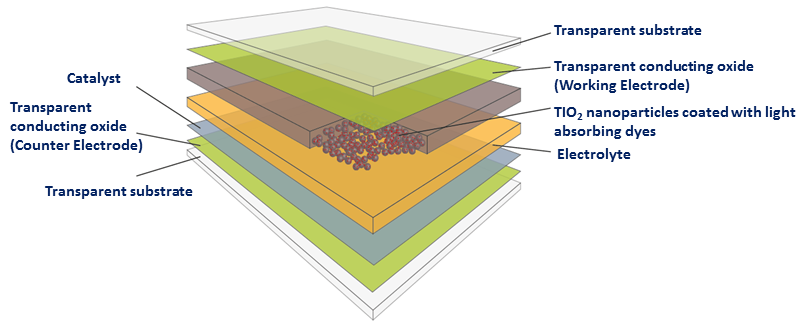
\includegraphics[width=\textwidth]{images/DSCs_struc}
\caption{Structure of a DSC }
\label{fig:DSC_struc}
\end{center}
\end{figure}

The most commonly used substrate is glass coated with \ac{FTO}. Attached to the surface of the nano-crystalline particles of Titanium dioxide(\ce{TiO2}) is a mono-layer of the light-sensitive-charge-transfer dye.The dye absorbed photons of incoming light and uses this energy to release free electrons to the \ce{TiO2} layer acting as the \ac{WE} and then onto metal contacts. An electrolyte is filled between the electrodes and helps transfer electrons from the \ac{CE} to the dye particle{which is in an oxidized state due to a loss of electron} to reduce it back to its ground state.The most commonly used redox couple, and the one that gives the best cell efficiencies when combined with \ce{TiO2}, is iodide/triiodide (\ce{I-}/\ce{I3-}). The oxidized dye gets electrons from the iodide ions which, in turn, get oxidized to triiodide in the process. The triiodide ions then diffuse to the counter electrode, where they get reduced back to iodide by the electrons returning from the external load. Thus, the cell operation is based on consecutive reduction/oxidation cycles and, in an ideal cell, no chemical substances are permanently transmuted. The most often used counter electrode catalyst for the triiodide/iodide reduction reaction is platinum, though also carbon materials and certain conductive polymers have been successfully employed in this function.\\
\begin{figure}[H]
\begin{center}
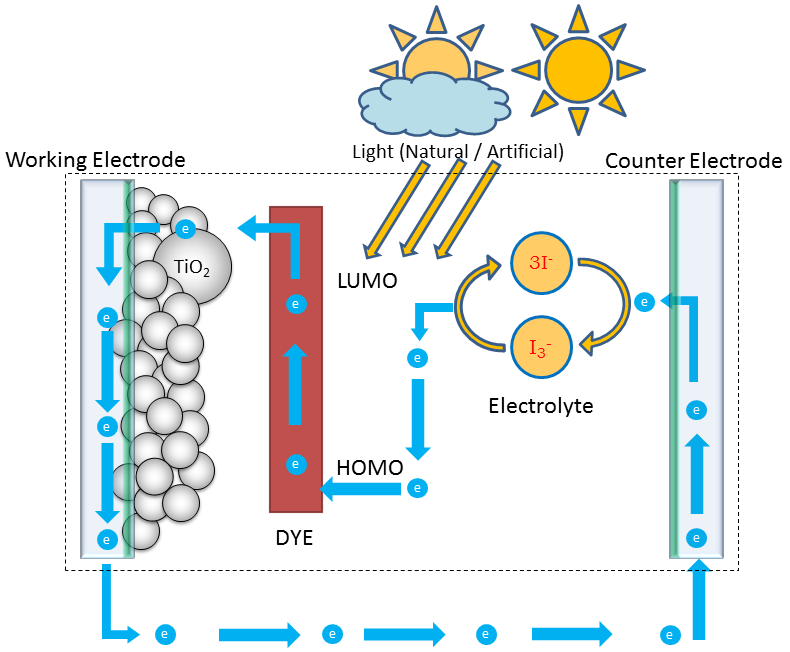
\includegraphics[width=\textwidth]{images/Cell_Cycle}
\caption{ The structure and operating principle of a DSC (adapted from \cite{toivola2010dye,}\cite{gcell_DSSC_cycle})}
\label{fig:Cell_Cycle}
\end{center}
\end{figure}

The amount of current that the cell is able to generate is determined by the energetic distance of the \ac{HOMO} and \ac{LUMO} of the dye, which equals the band gap in inorganic semiconductors. The maximum voltage, on the other hand, is defined as the difference between the redox level of the electrolyte and the Fermi level of the \ce{TiO2}.With iodide/triiodide redox couple, this difference is 0.9 V, though slight variation is caused by the electrolyte composition due to species adsorbed on the \ce{TiO2} surface, which may alter the Fermi level position somewhat. Also, there is always some recombination in the cell which lessens the amount of electrons in the TiO2 film, thus lowering the Fermi level and decreasing the cell voltage. \cite{toivola2010dye}.  This operating principle of \ac{DSCs} is depicted in the Figure ~\ref{fig:Cell_Cycle} on page ~\pageref{fig:Cell_Cycle}. \\


**Info about single diode model od DSCs Pictures etc** \newline



 \subsection{Advantages of DSCs }
  
  The *** of solar cells is slow **.A major contributing factor for this is the predominant type of solar cells used today -ones made from silicon, which are quite expensive and are complex to manufacture. This has lead to intensive research in to alternative solar cells in the past decade. \ac{DSCs} have many advantages over their 1st and 2nd generation counterparts. They offer transparency, low cost, and high power conversion efficiencies under cloudy and artificial light conditions.\ac{DSCs} work even in low-light conditions such as non-direct sunlight and cloudy skies.They are easy and economical to manufacture,with the major constituent materials available in abundance in most counties. **This availability of Raw material also enables us to scale the manufacturing to Tera-Watts levels relatively simple.Since raw-materials are non-toxic and there are no noxious emissions during manufacturing-Sustainable**\\
  
 
  
  
  \begin{figure}[H]
  \begin{center}
  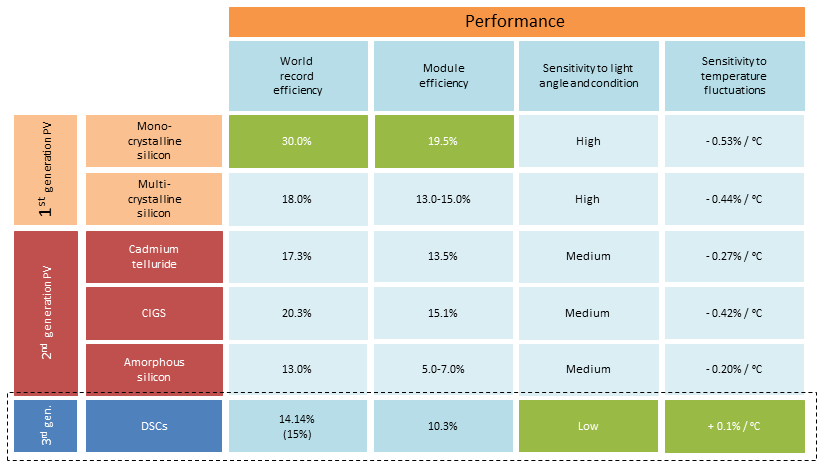
\includegraphics[width=\textwidth]{images/3rd_gen}
  \caption{ Three generations of cells –  Performance}
  \label{fig:3rd_gen}
  \end{center}
  \end{figure}
 
 \subsection{Modelling of te solar cell } 
  **Add more details about Advantage of DSC over conventional cells **\\
 
   
\section{Maximum power Point Tracking(MPPT)}

A photovoltaic (PV) array that functions under uniform radiation and temperature conditions presents an I–V and P–V characteristic as the one shown in Figure ~\ref{fig:IVgraph} and Figure ~\ref{fig:PVgraph},respectively. As can be observed, there is a single point, called \ac{MPP}, where the array provides the maximum power possible for these environmental conditions (radiation and temperature), and so functions with the maximum performance. When a load is connected directly to a PV array (direct coupling), the operation point is defined by the intersection of its I–V characteristics, as shown in Figure ~\ref{fig:IVgraph}. In general, this operation point does not coincide with the \ac{MPP}. Thus, in direct coupling systems, the array must be over-dimensioned to guarantee the power demand of the load. Obviously, this implies a more expensive system. To solve this problem, a DC/DC  converter with an algorithm for the automatic control of its duty cycle “${\delta}$” is inserted between the photovoltaic array and the load , resulting in what is known as \ac{MPPT} system. The MPPT must control the voltage or current (through the ${\delta}$ the converter) of the PV array regardless of the load, trying to place it in the \ac{MPP}.Therefore,the MPPT must find the optimal ${\delta}$ for the operation point of the PV array to coincide with the \ac{MPP}\cite{enrique2010reliable}.\\

Although the solution to operating in the \ac{MPP} may seem immediate, it is not. This is because the location of the \ac{MPP} in the I–V curve of the PV array is not known a priori. This point must be located, either by mathematical calculations over a valid model, or by using some search algorithm. This implies even more difficulty if we consider the fact that the \ac{MPP} presents non-linear dependencies with temperature and radiation\cite{enrique2010reliable}\\





  \begin{figure}[H]
  \begin{center}
  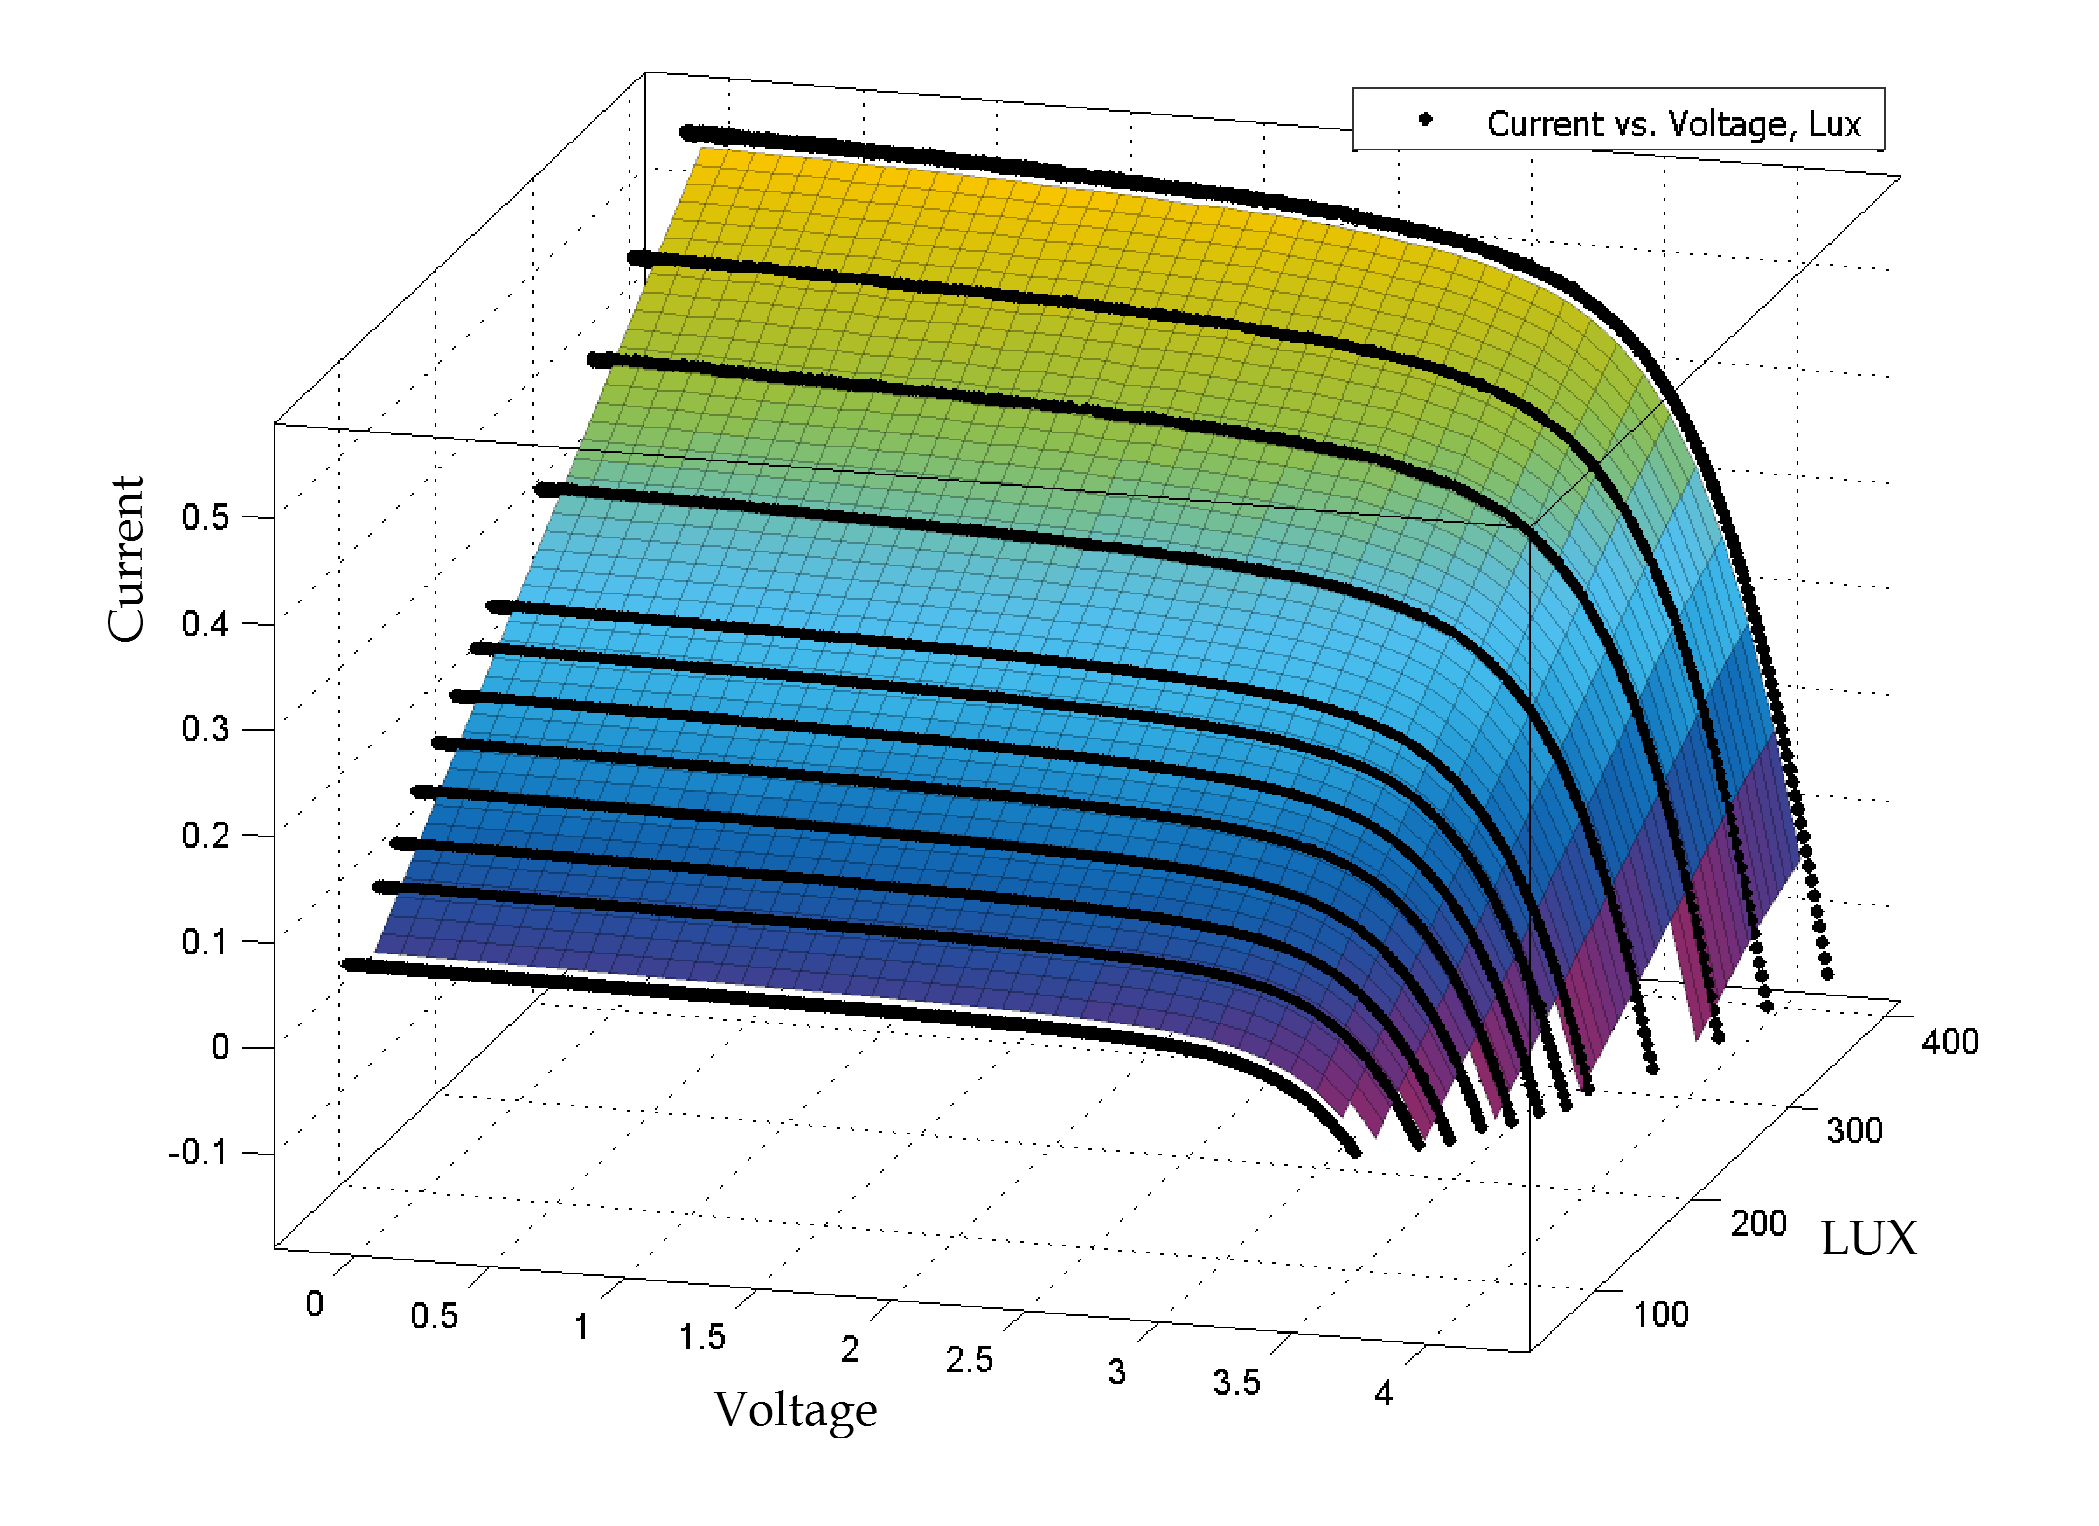
\includegraphics[width=\textwidth]{images/I-V-lux}
  \caption{I-V-Lux}
  \label{fig:IVgraph}
  \end{center}
  \end{figure}
  
    \begin{figure}[H]
    \begin{center}
    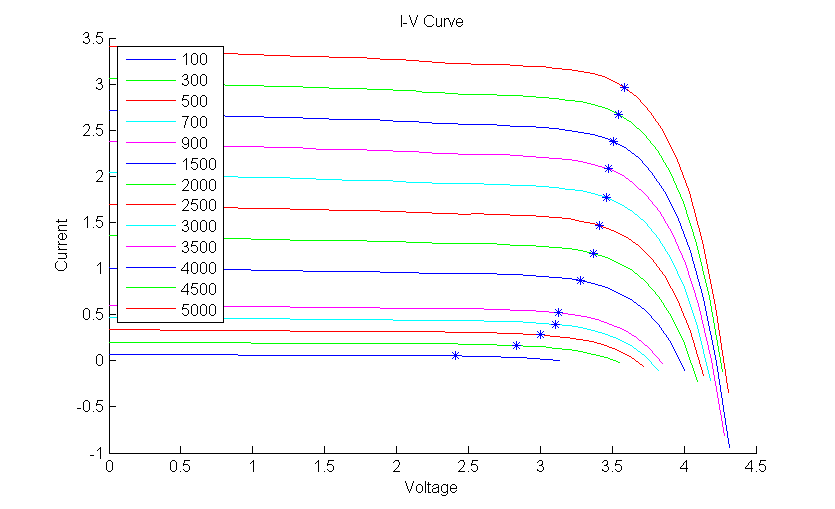
\includegraphics[width=\textwidth]{images/IV_lux_MPP}
    \caption{I-V Graph, MPPT marked with '*'}
    \label{fig:IV_mppgraph}
    \end{center}
    \end{figure}
  
  \begin{figure}[H]
  \begin{center}
  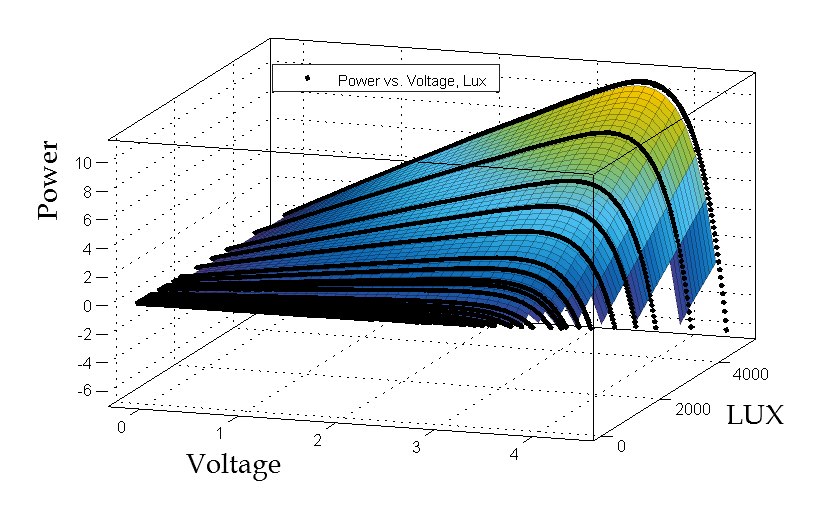
\includegraphics[width=\textwidth]{images/PV_LUX}
  \caption{ P-V Lux}
  \label{fig:PVgraph}
  \end{center}
  \end{figure}

As such, many \ac{MPPT} methods have been developed and implemented. The methods vary in complexity, sensors required, convergence speed, cost, range of effectiveness, implementation hardware, popularity, and in other respects. They range from the almost obvious (but not necessarily ineffective) to the most creative (not necessarily most effective). In fact, so many methods have been developed that it has become difficult to adequately determine which method, newly proposed or existing, is most appropriate for a given PV system.\\

  \subsection{Perturb and Observe Method }
  The \ac{PnO} Method is most widely used in \ac{MPPT} because of  its simple structure and it requires only few parameters. Figure ~\ref{fig:PnOflow}  shows the flow chart of \ac{PnO} method. It perturbs the PV array's terminal voltage periodically, and then it compares the PV output power with that of the previous cycle of perturbation. When PV power and PV voltage increase at the same time and vice versa, a perturbation step size, ${\Delta}$D will be added to the duty cycle, D to generate the next cycle of   perturbation in order to force the operating point moving towards the \ac{MPP}. When PV power increases and PV voltage decreases and vice versa, the perturbation step will be subtracted for the next cycle of perturbation.This process will be carried on continuously until \ac{MPP} is reached.However, the system will oscillate around the \ac{MPP} throughout this process, and this will result in loss of energy. These oscillations can be minimized by reducing the perturbation step size but it slows down the \ac{MPP} tracking system \cite{ngan2011study}.  \\
  
  \begin{figure}[H]
    \begin{center}
    
\includegraphics[width=\textwidth]{images/pacehold}
    \caption{ Flow chart for the Perturb and Observe Method }
    \label{fig:PnOflow}
    \end{center}
    \end{figure}
  
  \subsection{Incremental Conductance Method }
  The  solar array terminal  voltage  can  be  adjusted relative to the MPP voltage by measuring the incremental and instantaneous  array  conductance (dI/dV and I/V ,   respectively).  Although  the  incremental  conductance method offers good performance under rapidly changing atmospheric  conditions,  four  sensors  are  required to   perform the  computations. The  drawback is that sensor devices require  more  conversion  time  thus  result in a large amount of power loss.   \\
  
   \begin{figure}[H]
      \begin{center}
      
\includegraphics[width=\textwidth]{images/pacehold}
      \caption{ Flow chart for the Incremental Conductance Method}
      \label{fig:inCflow}
      \end{center}
      \end{figure}
  \subsection{fractional open circuit voltage Method }
  This is a method based on the linear relationship between output voltage of the PV array at the \ac{MPP}, V\textsubscript{MPP} and the PV array's open circuit voltage, V\textsubscript{OC} in under varying temperature and solar irradiance. \\
  
  \begin{equation}
    \begin{aligned}
  V\textsubscript{MPP}\approx k\textsubscript{i}V\textsubscript{OC}
  \label{eq:equ_fracoc}
  \end{aligned}
  \end{equation}
  
  Constant value of k\textsubscript{i} is dependent on the characteristics of PV array. Generally, it has to be computed empirically in order to determine the V\textsubscript{MPP} and V\textsubscript{OC} for varied temperatures and solar irradiances. The value of k\textsubscript{i} ranges from 0.73 to 0.80  for most PV modules over a temperature range of 0 to 60$^\circ$C.Figure ~\ref{fig:focflow} describes the operation of a \ac{FOCV}, the PV array is temporarily isolated from \ac{MPPT},then the open circuit voltage, V\textsubscript{OC} is measured periodically by shutting down the power converter momentarily. The \ac{MPPT} calculates V\textsubscript{MPP} from the pre-set value of k1 and the calculated value of V\textsubscript{OC}. Then, the array's voltage is varied until V\textsubscript{MPP} is  reached . The shut-down of power converter periodically will incur temporary loss of power which results in power extracted will not be the maxima. Since is an approximation, the PV array will never reach the \ac{MPP}. Even though this technique is very easy and cheap for implementation, yet since true \ac{MPP} is never reached there is always a loss in power during operation\cite{ngan2011study}.
  
  \begin{figure}[H]
        \begin{center}
        
\includegraphics[width=\textwidth]{images/pacehold}
        \caption{ Flow chart for the fractional open circuit voltage Method  Method }
        \label{fig:focflow}
        \end{center}
        \end{figure}
  
\subsection{other Algorithms}
  \begin{itemize}
  \item {\bf Fixed duty cycle} The fixed duty cycle represents the simplest of the methods and it does not require any feedback, where the load impedance is adjusted only once for the maximum power point and it is not adjusted again.
  \item {\bf Pilot cell} In the pilot cell MPPT algorithm, the constant voltage or current method is used, but the open-circuit voltage or short-circuit current measurements are made on a small solar cell, called a pilot cell, that has the same characteristics as the cells in the larger solar array The pilot cell measurements can be used by the MPPT to operate the main solar array at its MPP, eliminating the loss of PV power during the V\textsubscript{OC} or I\textsubscript{sc} measurement
  \item {\bf Fractional short-circuit current }  under varying atmospheric conditions, I\textsubscript{MPP} is approximately linearly related to the I\textsubscript{SC} of the PV array. \newline
    \begin{equation}
      \begin{aligned}
    I\textsubscript{MPP} \approx k\textsubscript{j}I\textsubscript{SC}
    \label{eq:equ_fracoc}
    \end{aligned}
    \end{equation}
   \item {\bf Fuzzy logic controller} (FLC) have the advantages of working with imprecise inputs, it does not need an accurate mathematical model and it can handle non-linearity as well.
  \end{itemize} 
  
\subsection{Proposed MPPT Algorithm}
  insert text here insert text here insert text here insert text here insert text here
  insert text here insert text here insert text here insert text here insert text here insert text here insert text here insert text here insert text here insert text here insert text here insert text here insert text here insert text here insert text here insert text here insert text here insert text here insert text here insert text here insert text here insert text here insert text here insert text here   \\
  
  \begin{figure}[H]
   \begin{center}
   
\includegraphics[width=\textwidth]{images/pacehold}
   \caption{ Flow chart for Proposed MPPT Algorithm }
   \label{fig:cyflow}
   \end{center}
  \end{figure}


\section{Scope, Thesis Goals and Objectives}

This thesis focuses on the finding a practically **optimal** and usable \ac{MPPT} algorithm that is optimised to be used with the current \ac{DSCs}.\\


The objectives of the thesis can be summarized as:
\begin{itemize}

\item Develop an Electrical model for DSCs and verify the accuracy of said model.
 
\item Compare and optimize the following Maximum power point tracking (MPPT) algorithms for compatibility with the above Model using MATLAB{\textregistered} and Simulink{\textregistered}.
	\begin{enumerate}
		\item Perturb and Observe (\ac{PnO}) Method.
		\item Incremental Conductance Method (\ac{ICM}).
		\item fractional open circuit voltage (\ac{FOCV}) Method.
		
	\end{enumerate}
\item Setting up the test environment   
\item Execution of test cases on prototype developed, based on two of the best optimized algorithm, with recordable test results.
\item Develop Reference designs for production.
\item Internal report.
\item  Master thesis report. 
\end {itemize}

\section{Thesis outline}
\begin{itemize}
\item Chapter 1 Presents the background and the main objectives of this thesis \\
\item Chapter 2 Contains the prior research and literature that this thesis was based on, it also discusses the principle of operating principles/state-of-the-art  of \ac{DSCs} and of \ac{MPPT} \\
\item Chapter 3 concerns the  research methods, measurement techniques and implementation of the thesis.
\item Chapter 4 Gives a summary of the results. 
\item The thesis is Concluded and Future Work talked about in Chapter 5
\end {itemize}

\section{Research Methodology}
The implementation of the thesis is ** 
\begin{itemize}
\item Develop a suable model for the \ac{DSCs} based on either:.
	\begin{enumerate}
		\item the single diode equation for \ac{DSCs}.
		\item based on experimental modelling Methods .
	\end{enumerate}
\item objective study of current algorithms;  weigh their pros vs cons.
\item Validation of the Model and algorithm in MATLAB{\textregistered} and Simulink{\textregistered}.
\item Implementation in test Hardware .
\end {itemize}